\section{Classification \& Bio-geophysical Parameter Retrieval}
\label{sec:task2}

\subsection{Can we predict where there is chlorophyll through classification?}
\label{sec:classify}

We will use \textit{K-Means clustering} to classify the data. K-means clustering is a 
unsupervised learning algorithm that can be used to classify and cluster data into $k$ 
different clusters. The data points are adjusted iteratively until all points are 
associated with the nearest cluster. We want to cluster each observation (pixels, with $n$ spectral channels) into a specific 
cluster (environment class, ie. deep water, shallow water, vegetation). 


\begin{figure}
    \centering
    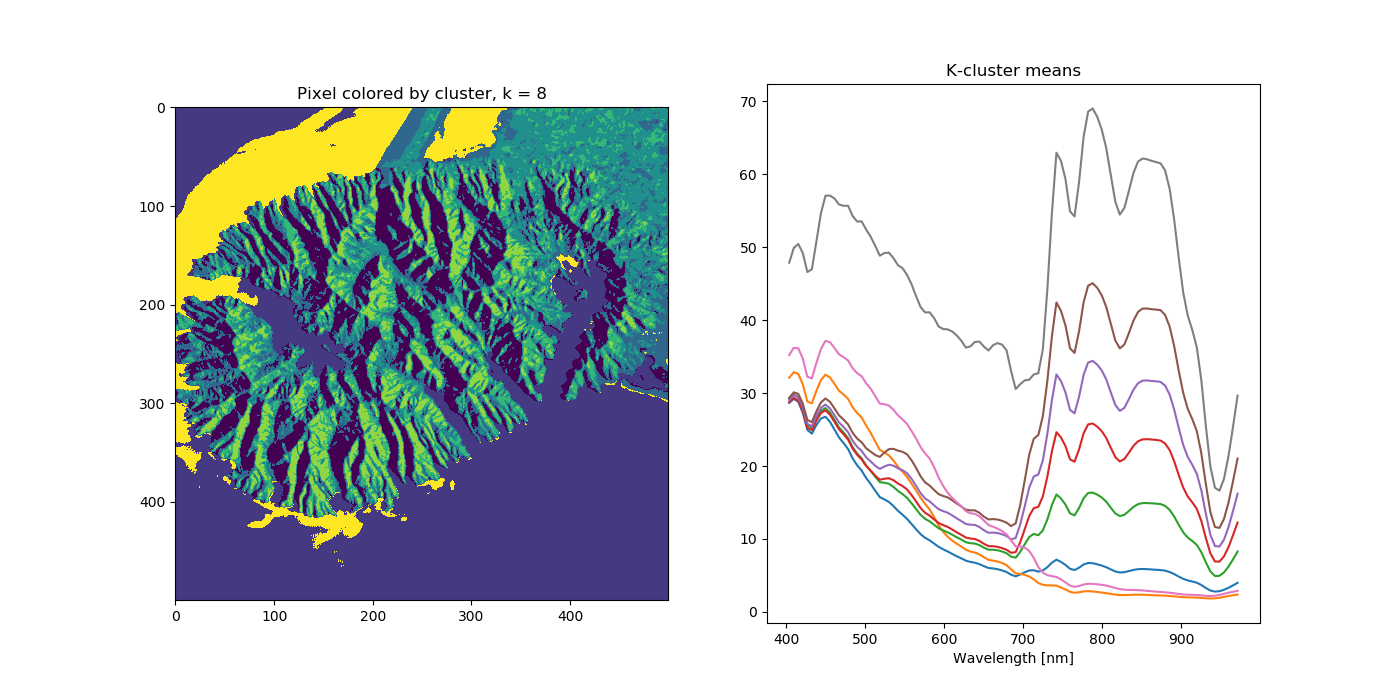
\includegraphics[width=\textwidth]{../fig/kmean/kmean_8.png}
    \caption{K-mean clusters of the image}
    \label{fig:kmean}
\end{figure}

As we can see from \cref{fig:point_spectra}, we know that those three different points 
have distinctly different spectra, thus it should be possible to classify them accordingly. 
The results of a K-mean clustering, run with Spectral Python's \textit{kmeans} function \cite{website:spectral}, 
can be seen in \cref{fig:kmean}. We clearly see different classes for water, land, and vegetation, the latter 
containing lots of chlorophyll. We also see a very distinct class along the coast on the upper part 
of the image. This may very well be a collection of chlorophyll, but it might also just be shallow water, or 
more likely a combination of both. 

\subsection{How well can we directly estimate the chlorophyll content?}

We use the NASA OBPG algorithm, defined in equation 4 in the assignment 
\cite{assignment}, as well as the parameters given there, to try to 
visualize the chlorophyll contents. Using the closest available wavelengths 
in the dataset, $\lambda_{green} = 553$ (i = 26) and $\lambda_{blue} = [444, 490, 507]$ 
(i = [7, 15, 18]). The results can be seen in \cref{fig:obpg}. We can clearly 
see high concentrations on the north west coast (assuming north is at the 
top of the image), same place as in \cref{fig:kmean}, but now we also see 
quite a bit on the southern coast as well. Thus it seems that this 
algorithm performs better than the k-means clustering. 

\begin{figure}[h!]
    \centering
    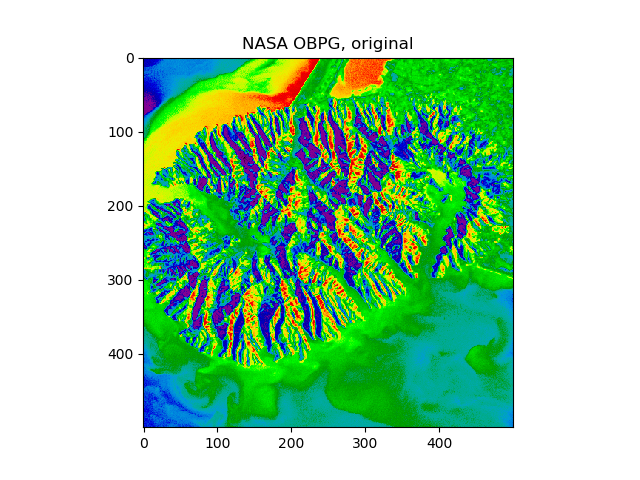
\includegraphics[width=\textwidth]{../fig/NASA OBPG, original.png}
    \caption{Results from the NASA OBPG algorithm, showing chlorophyll concentrations 
    in the water}
    \label{fig:obpg}
\end{figure}

\subsection{How can we estimate the reflectance from the surface of the ocean?}
\label{sec:atmoshperic_cor}

The data in the HICO dataset actually contains the measurement of radiance exiting the top 
of the atmosphere, and not the radiance of the water directly. Therefore we must recover the 
radiance $R_{rs}$ of the water from the top of atmosphere (TOA) measurements. This is done with 
the empirical line (ELM) method, as described in \cite{assignment}, on the form \cref{eq:R_rs}. 
Where $a$ and $b$ are terms that model the absorption of light in the atmosphere, which is to 
be estimated, and $L$ is the measured value in the HICO dataset. 

\begin{equation}
    \label{eq:R_rs}
    R_{rs}(\lambda) = \frac{L(\lambda) - b(\lambda)}{a(\lambda)}
\end{equation}

\begin{figure}
    \centering
    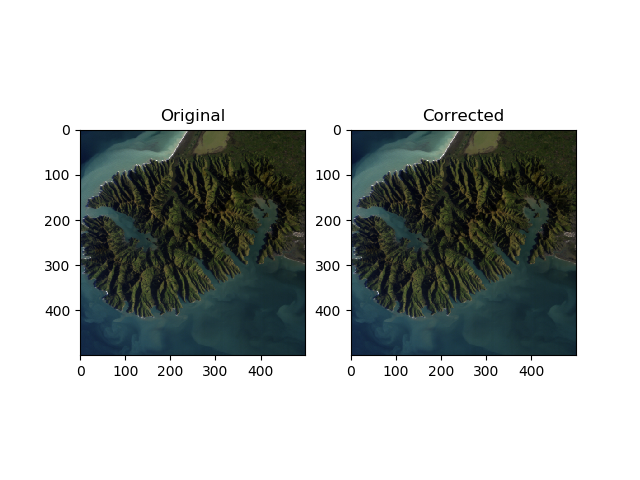
\includegraphics[width=\textwidth]{../fig/pseudo_rgb_corrected.png}
    \caption{Pseudo RGB image of the atmosphere corrected image}
    \label{fig:RGB_corrected}
\end{figure}

After performing the atmospheric correction, the resulting image is shown in 
\cref{fig:RGB_corrected}. It is very difficult to see a clear difference between 
the two by only looking at the image, but if we look at the pixel values for the red, 
green and blue channels separately, we see that the blue color channel is only about 2\% 
of the original, uncorrected pixel value, while the red and blue channels are about 9-10\% 
of their original values. Thus it would seem that the atmospheric correction removes some of 
the blue color of the image. 

\subsection{Compute chlorophyll concentration using atmosphere-corrected data}

After performing the atmospheric correction, as described in \cref{sec:atmoshperic_cor}, 
we perform the NASA OBPG algorithm again on the corrected image cube. As we can 
see from the results in \cref{fig:obpg_corrected}, it is quite different from the 
original results from \cref{fig:obpg}. The strong concentration we found at the north 
west coast of the original (\cref{fig:obpg}), is no longer to be seen in the corrected 
image. Instead, we see a high concentration of chlorophyll on the south eastern coast, 
as well as a small patch in the bay on the western part of the landmass. 
\todo{Rewrite after fixing images, colors are wrong}

\begin{figure}
    \centering
    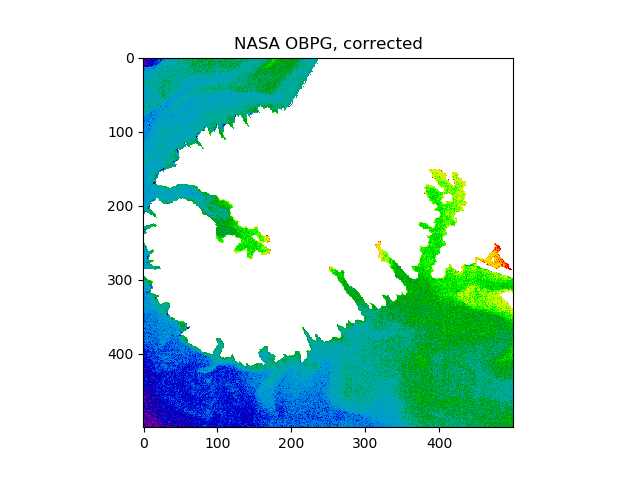
\includegraphics[width=\textwidth]{../fig/NASA OBPG, corrected.png}
    \caption{Results from the NASA OBPG algorithm using the atmospheric correction described 
    in \cref{sec:atmoshperic_cor}, showing chlorophyll concentrations in the water}
    \label{fig:obpg_corrected}
\end{figure}


\begin{figure}
    \centering
    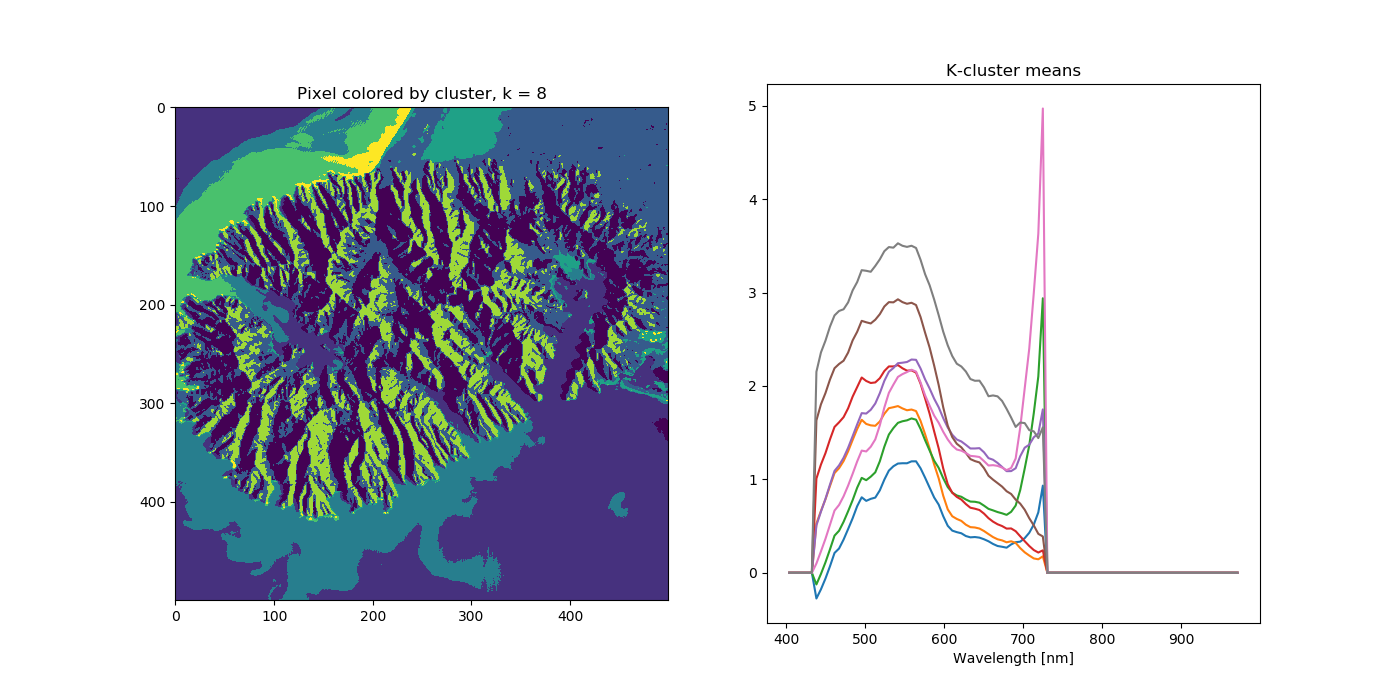
\includegraphics[width=\textwidth]{../fig/kmean/kmean_corrected8.png}
    \caption{K-mean clustering performed on the atmospheric corrected image cube}
    \label{fig:kmean_corrected}
\end{figure}



\subsection{Classify land versus water}
\label{sec:landmask}

We want to classify only the chlorophyll content of the water, we're not interested 
in looking at the land. Therefore we want to mask out the landmass and show only 
the water. We again use K-means clustering to classify the data into different 
classes. By performing it multiple times for varying numbers of classes and comparing 
the result from \cref{fig:kmean}, \cref{fig:kmean_corrected}, as well as all other 
iterations from 1-10 classes on both corrected and original data, we find that 
performing k-means clustering with 10 clusters on the atmospherically corrected 
image cube gives the best performance regarding classifying water vs land. Setting 
the max number of iterations to 100, the algorithm converges after around 80 iterations, 
giving a good result. 

After the k-means clustering is performed, we look at the spectral plot of the 
different classes. We know from \cref{sec:representative_spec} roughly how the 
spectra of water looks compared to land/vegetation. We the pick the spectral lines 
from the k-means result that most resemble the spectral lines of water, and we remove 
any lines that resemble those of land/vegetation. We then end up with a handful of 
different classes that represents water, and the rest is land. We set the pixel values 
of all points inside the water classes to 1, and all other pixels to 0 to create the 
mask. The mask itself is shown in \cref{fig:landmask}. When put over the image, we get 
\cref{fig:mask_rgb}.
\todo{Colors are wrong, fix code}


\begin{figure}[h!]
    \centering
    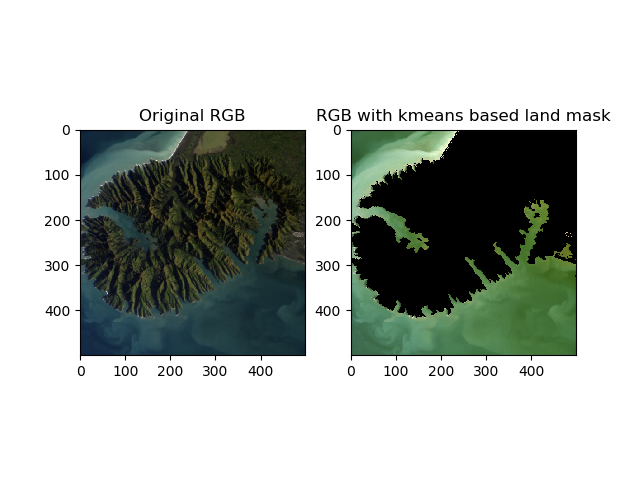
\includegraphics[width=\textwidth]{../fig/rgb_masked.png}
    \caption{Masking away the land area}
    \label{fig:mask_rgb}
\end{figure}

\begin{figure}[h!]
    \begin{minipage}{.5\textwidth}
        \centering
        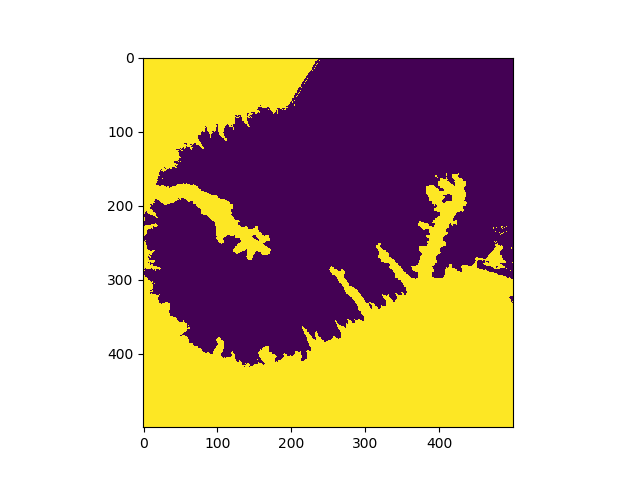
\includegraphics[width=\textwidth]{../fig/landmask.png}
        \caption{The mask found in \cref{sec:landmask}, based on kmeans clustering}
        \label{fig:landmask}
        \end{minipage}
        %\hspace{1.2cm}
    \begin{minipage}{.5\textwidth}
        \centering
        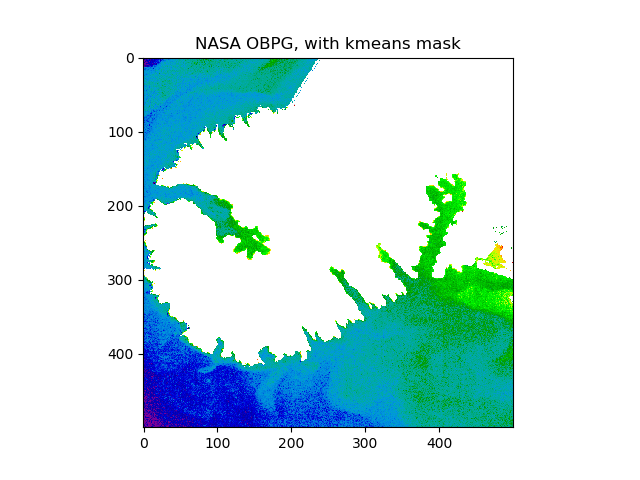
\includegraphics[width=1.5\textwidth]{../fig/NASA OBPG, with kmeans mask.png}
        \caption{Running the OBPG algorithm on the masked image, using mask from \cref{fig:landmask}}
        \label{fig:mask_obpg}
        \end{minipage}%
    \end{figure}


\subsection{Other bio-geophysical parameters}

In the available spectral measurements between 400-1000nm we may find several 
other kinds of bio-geophysical parameters. In general, bio-geophysical parameters 
include biological (plant species, interactions in the ecology, biotic 
productivity), geological (soil types, erosion), and physical (light, heat) \cite{website:esa_bio-geophysical}. 
Examples include detecting phytoplankton pigments and gelbstoff \cite{Lee:02}, or land degradation 
processes in semi-arid geographical areas \cite{Kaufmann2002}.

\subsection{Alternative atmospheric correction methods}

One of the drawbacks of using the empirical line method (ELM) is that it requires at 
least one field, laboratory, or other reference spectrum, preferably 2 or more like 
the 2 reference spectra used in this report (shallow and deep water) to create the 
linear regression used in removing the solar- and atmospheric path radiance. If such 
reference spectra, for all required wavelengths, is not available for the region of 
interest, this method can not be used. \cite{Karpouzli2003} 

There exists a whole lot of different atmospheric correction tools and algorithms. 
Harris Geospatial lists 9 different tools available for ENVI \cite{website:harrisgeo}, 
including Dark Subtraction, Empirical Line, FLAASH, Flat Field, IAR, Log Residuals, 
QUAC, Thermal Atmospheric Correction, and Convert to Emissivity and Temperature. 

For instance, the Flat Field Correction algorithm can be easily implemented 
by normalizing the images to an area of known "flat" reflectance, where 
the average spectrum from a region of interest can be used as reference.